\documentclass[landscape]{beamer}

\usepackage{drawstack}

\title{Compiling C with Clang by examples
\\[1em]
\(
 C \stackrel{\mbox{Clang}}{\longrightarrow} x86
 \)
 }
\author{Hayo Thielecke
\\
University of Birmingham
\\
\url{http://www.cs.bham.ac.uk/~hxt}
}


\begin{document}

\begin{frame}{}
\maketitle
\end{frame}

\begin{frame}{Contents}
\tableofcontents
\end{frame}

\section{Introduction}

\begin{frame}{Structure of the module}

\begin{block}{Parsing \checkmark}
\begin{itemize}
\item Progression from: Language + Logic, Models of Computation
\item abstract machines, formal,``mathy''
\end{itemize}
\end{block}

\begin{block}{Compiling C with Clang}
\begin{itemize}
\item Progression from: Computer Systems + Architecture, C/C++
\item not so formal, by example, x86 machine code
\end{itemize}
\end{block}

\begin{block}{Implementing functional languages}
\begin{itemize}
\item Progression from: functional programming
\item builds on abstract machines and C stack
\end{itemize}
\end{block}

\end{frame}
\begin{frame}[fragile]{Example}

\begin{minipage}{.5\textwidth}
C code
\begin{verbatim}
long f(long x, long y)
{
  long a, b;
  a = x + 42;
  b = y + 23;
  return a * b;
}
\end{verbatim}
\end{minipage}
%
\begin{minipage}{.4\textwidth}
x86 generated by Clang
\begin{verbatim}
f:                                      
	addq	$42, %rdi
	leaq	23(%rsi), %rax
	imulq	%rdi, %rax
	ret
\end{verbatim}
\end{minipage}
\vspace{2em}

The assembly code does not look much like the source code.
 
%How did the compiler know what to generate?

What happened to variables?

What happened to types?
\end{frame}

\begin{frame}{These are open source lectures and notes}

The \LaTeX{} source is in

\url{https://github.com/hayo-thielecke/clang-lectures}

\texttt{c-clang.tex} is for my slides

\texttt{c-clang-notes.tex} is for collaborative note taking.

\end{frame}

\begin{frame}{Aims and overview}

\begin{itemize}
\item
We will see some typical C code compiled to x86 assembly by LLVM/Clang
\item Emphasise general principles used in almost all compilers
\item Use Clang on C and x86 for example and concreteness
\item
\alert{What} Clang does, not details of \alert{how} it does it internally
\item
Enough to compile some C code by hand line by line
\item
C language features $\mapsto$ sequence of assembly instructions + addresses
\item
Various language features on top of vanilla functions
\item
Optimizations

\end{itemize}

\end{frame}

\section{Clang, LLVM, and x86 subset}

\begin{frame}{Clang and LLVM, the bestest and mostest compiler}

Clang is the bestest C/C++ compiler

\url{http://clang.llvm.org}

LLVM  is the mostest compiler infrastructure

\url{http://llvm.org}

Apple uses it

\url{https://developer.apple.com/xcode/}

Many projects, for example:

Emscripten: An LLVM to JavaScript Compiler

Rust: ``a safe, concurrent, practical language'' (as per blurb)

A not too technical intro to LLVM:
\url{http://www.aosabook.org/en/llvm.html}

\end{frame}

\begin{frame}{Using Clang}

Please do experiments yourself for seeing how LLVM/Clang compiles C.

Clang comes with XCode on OS X.

If you do not have LLVM on your computer:

ssh into a lab machine and type 

module load llvm/3.3

To compile, type

clang -S test.c

Then the assembly code will be in test.s

Function frodo will be labelled frodo: in test.s

For optimization, use

clang -S -O3 test.c

\end{frame}


%\section{Target architecture}

\begin{frame}{Target architecture for Clang output}

We will only need a tiny subset of assembly.

Quite readable.

Instruction we will need:

\[
\texttt{mov push pop call ret jmp add mul test be lea}
\]

The call instruction pushes the current instruction pointer onto the stack as the return address

ret pops the return address from the stack and makes it the new instruction pointer

A nice target architecture should have lots of general-purpose registers with indexed addressing.

Like RISC, but x86 is getting there in the 64-bit architecture

\end{frame}

\begin{frame}{Assembly generated by clang is x86 in AT\&T syntax}

mov syntax is target-last:

\texttt{mov} x y is like y = x ;

r prefix on registers means 64 bit register

movq etc: q suffix means quadword = 64 bits

\texttt{\%} register

\texttt{\$} constant

\texttt{\%rbp} = base pointer = frame pointer in general terminology

\texttt{\%rsp} = stack pointer, push and pop use it

indexed addressing \texttt{-24(\%rbp)}

\end{frame}


\begin{frame}[fragile]{Typical C code to compile}
\begin{minipage}{.5\textwidth}
\begin{verbatim}
long f(long x, long y)
{
  long a, b;
  a = x + 42;
  b = y + 23;
  return a * b;
}
\end{verbatim}
\end{minipage}
%
\begin{minipage}{.4\textwidth}
Parameters/arguments:
\\
 x and y

Local/automatic variables
\\
 a and b 
\end{minipage}
\\[4em]

More precisely, x and y are \emph{formal} parameters.

In a call f(1,2), 1 and 2 are the \emph{actual} parameters.

We will use the words ``parameter'' and ``argument'' interchangeably.

\end{frame}

\begin{frame}{Two big ideas in compiling functions}

\begin{block}{stack $\leftrightarrow$ recursion}

compare: parsing stack

many abstract and not so abstract machines use stacks

including JVM

In C: one stack frame per function call
\end{block}

\begin{block}{Names $\to$ indices}
Names can be compiled into indices, discovered many times

%deBruijn indices: lambda calculus without variables
%
%cartesian closed categories, CAM machine for CAML

In C: variables become small integers to be added to the base pointer

\end{block}

\end{frame}

\section{Call stack and stack frames}

\begin{frame}[fragile]{Stack frame details}

The details differ between architectures (e.g., x86, ARM, SPARC)

Ingredients of stack frames, in various order, some may be missing:

return address 

parameters

local vars

saved frame pointer

caller or callee saved registers

static link (in Pascal and Algol, but not in C)

this pointer for member functions (in C++)
\end{frame}


\begin{frame}[fragile]{A traditional stack layout (but not Clang)}

%On most hardware, the stack grows towards smaller addresses.

Convention: we draw the stack growing \alert{downwards} on the page. 

Suppose function \texttt g calls function \texttt f.


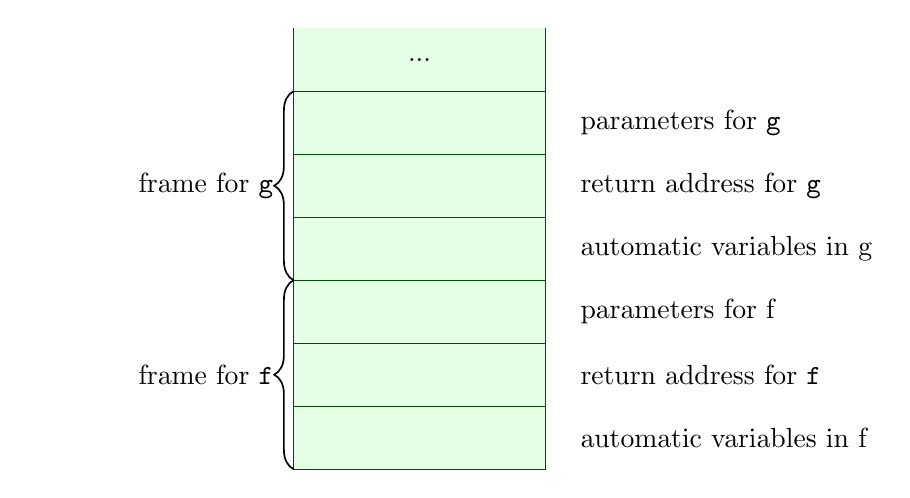
\begin{tikzpicture}[scale=.8]
  \stacktop{}
  \startframe
      \cell{}  
\cellcom{parameters for \texttt g} 
    \cell{}  
\cellcom{return address for \texttt g} 
      \cell{}        
    \cellcom{automatic variables in g}         
\finishframe{frame for \texttt g\ } 
  \startframe
  \cell{}  
    \cellcom{parameters for f} 
  \cell{}  
\cellcom{return address  for \texttt f} 
  \cell{}  
    \cellcom{automatic variables in f}
 \finishframe{frame for \texttt f\ } 
\end{tikzpicture}
There may be more in the frame, e.g. saved registers  
\end{frame}   


\begin{frame}[fragile]{What about recursive functions?}

Consider the standard example of recursion:

\begin{verbatim}
long factorial(long n)
{
  if(n == 0)
    return 1;
  else
    return factorial(n - 1) * n;
}
\end{verbatim}


\end{frame}

\begin{frame}[fragile]{Call stack: one frame per function \alert{call}}

Recursion example: fac(n) calls fac(n - 1). Each recursive call gets a smaller parameter.

The return address points into the code segments, \alert{not the stack} or heap.

What are the return addresses?
\\[1em]

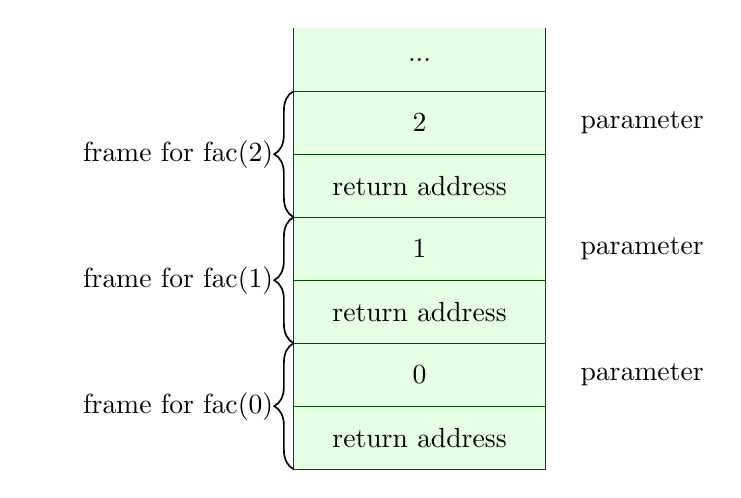
\begin{tikzpicture}[scale=.8]
  \stacktop{}
    \startframe
      \cell{2}  
    \cellcom{parameter}
  \cell{return address}  
  \finishframe{frame for {fac(2)}} 
  \startframe
      \cell{1}  
    \cellcom{parameter}
  \cell{return address}  
  \finishframe{frame for {fac(1)}} 
  \startframe
  \cell{0}  
    \cellcom{parameter} 
  \cell{return address}  
 \finishframe{frame for fac(0)} 
\end{tikzpicture}

\end{frame}   

\begin{frame}[fragile]{Return address example}

\begin{verbatim}
long factorial(long n)
{
  if(n == 0)
    return 1;
  else
    return factorial(n - 1) * n;
}
\end{verbatim}

The return address is a pointer to the compiled code. The returned value is returned into the hole $\bigcirc$ position in the last statement,
\[
\texttt{return $\bigcirc$ * n;}
\]
Thus when the function returns, 1 is plugged into the hole, then 2, then 6, \ldots

The return address represents a continuation.
\end{frame}

\begin{frame}{Calling conventions and stack frame layout}

The calling convention differs between compilers and architectures

Old school: 
\\push arguments onto stack, then do a call instruction (which pushes return address)

Modern architectures have many registers
\\
$\Rightarrow$ pass arguments in registers when possible; Clang does this

Some RISC architectures put return address into a link register

more exotic: SPARC has register windows for parameter passing
\end{frame}


\begin{frame}[fragile]{Stack frame in clang C calling convention on x86}

Clang \alert{passes parameters in registers} \texttt{rdi}, \texttt{rds}, \ldots

The parameters \alert{also have a slot in the frame}

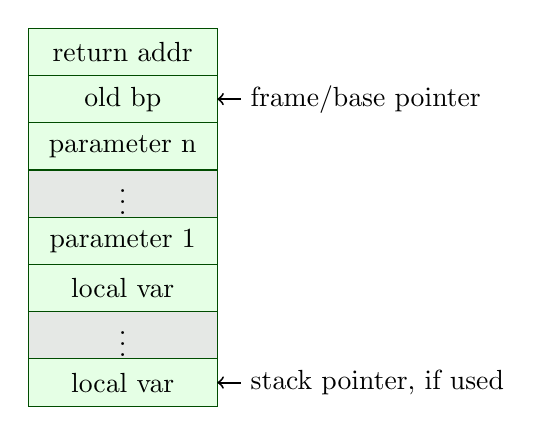
\begin{tikzpicture}[scale=.6]
  \startframe
     \cell{return addr} 
    \cell{old bp}  \cellptr{\textrm{frame/base pointer}} 
      \cell{parameter n}
     \cell[padding]{\vdots}
         \cell{parameter 1} %\cellptr{\texttt{stack} + 2}
    \cell{local var}
     \cell[padding]{\vdots}
    \cell{local var}\cellptr{\textrm{stack pointer, if used}} 
%\finishframe{array} 
\end{tikzpicture}
  
\end{frame} 


\begin{frame}[fragile]{Clang function idiom}

\url{http://llvm.org/docs/LangRef.html#calling-conventions}

\begin{verbatim}
f:
	pushq	%rbp
	movq	%rsp, %rbp
    ... body of function f
	popq	%rbp
	ret
\end{verbatim}

parameters are passed in registers rdi, rsi

return value is passed in register rax
\end{frame}



\begin{frame}[fragile]{Computing the index in the frame}

Simple in principle: 
\\
walk over the syntax tree and keep track of declarations

The declarations tell us the size: long x means x needs 8 bytes

That is why C has type declarations in the first place

\begin{verbatim}
long f(int x, int y) // put y at -8 and x at -16
{
    int a;    // put a at -24
    int b;    // put b at -32
    a = x;    // now we know where a and x are 
              // relative to rbp
}    
\end{verbatim}

Exercise: what happens if we also have char and float declarations?    
\end{frame}

\begin{frame}[fragile]{Clang stack frame example}
\begin{verbatim}
long f(int x, int y) // put y at -8 and x at -16
{
    int a;    // put a at -24
    int b;    // put b at -32
    ...
}
\end{verbatim}
  
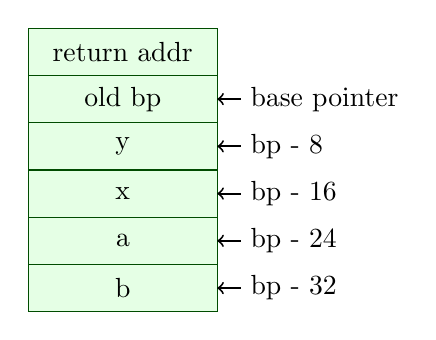
\begin{tikzpicture}[scale=.6]
 % \startframe
     \cell{return addr} 
    \cell{old bp}  \cellptr{\textrm{base pointer}} 
      \cell{y}\cellptr{\textrm{bp - 8}}
         \cell{x} \cellptr{\textrm{bp - 16}}
    \cell{a}  \cellptr{\textrm{bp - 24}}
    \cell{b} \cellptr{\textrm{bp - 32}}
% \finishframe{array} 
\end{tikzpicture}
  
\end{frame} 


\begin{frame}[fragile]{Compiled with clang -S}
\begin{minipage}{.55\textwidth}
\begin{verbatim}
long f(long x, long y)
{
  long a, b;
  a = x + 42;
  b = y + 23;
  return a * b;
}
\end{verbatim}

\begin{eqnarray*}
\texttt y&\mapsto& \texttt{rdi}
\\
\texttt x&\mapsto& \texttt{rsi}
\\
\texttt y&\mapsto& \texttt{rbp}-8
\\
\texttt x&\mapsto& \texttt{rbp}-16 
\\
\texttt a&\mapsto& \texttt{rbp}-24
\\
\texttt b&\mapsto& \texttt{rbp}-32
\end{eqnarray*}

\end{minipage}
%
\begin{minipage}{.4\textwidth}
\begin{verbatim}
f:
	pushq	%rbp
	movq	%rsp, %rbp
	movq	%rdi, -8(%rbp)
	movq	%rsi, -16(%rbp)
	movq	-8(%rbp), %rsi
	addq	$42, %rsi
	movq	%rsi, -24(%rbp)
	movq	-16(%rbp), %rsi
	addq	$23, %rsi
	movq	%rsi, -32(%rbp)
	movq	-24(%rbp), %rsi
	imulq	-32(%rbp), %rsi
	movq	%rsi, %rax
	popq	%rbp
	ret
\end{verbatim}
\end{minipage}
\end{frame}



\begin{frame}[fragile]{Optimization: compiled with clang -S -O3}
\begin{minipage}{.5\textwidth}
\begin{verbatim}
long f(long x, long y)
{
  long a, b;
  a = x + 42;
  b = y + 23;
  return a * b;
}
\end{verbatim}
\end{minipage}
%
\begin{minipage}{.4\textwidth}
\begin{verbatim}
f:                                      
	addq	$42, %rdi
	leaq	23(%rsi), %rax
	imulq	%rdi, %rax
	ret
\end{verbatim}
\end{minipage}
\end{frame}

\begin{frame}[fragile]{Many arguments}
Some passed on the stack, not in registers. These have positive indices. Why?
\\[2em]

\begin{minipage}{.6\textwidth}
\begin{verbatim}
long a(long x1, long x2, 
long x3, long x4, long x5, 
long x6, long x7, long x8)
{
  return x1 + x7 + x8;
}
\end{verbatim}
\end{minipage}
%
\begin{minipage}{.3\textwidth}
\begin{verbatim}
a:                             
	addq	8(%rsp), %rdi
	addq	16(%rsp), %rdi
	movq	%rdi, %rax
	ret
\end{verbatim}
\end{minipage}
\end{frame}


\end{document}

